%to-do
%add images
%add references
%do section 4


\documentclass[12pt, titlepage]{article}

\usepackage{fullpage}
\usepackage[round]{natbib}
\usepackage{multirow}
\usepackage{booktabs}
\usepackage{tabularx}
\usepackage{graphicx}
\usepackage{float}
\usepackage{hyperref}
\hypersetup{
    colorlinks,
    citecolor=black,
    filecolor=black,
    linkcolor=red,
    urlcolor=blue
}
\usepackage[round]{natbib}

\title{SE 3XA3: User Guide\\PasswordProtectionProgram}

\author{Team 28, Tuples1
		\\ Suhavi Sandhu (sandhs11)
		\\ Shabana Dhayananth (dhayanas)
		\\ Joseph Lu (luy89)
}

\date{\today}

\begin{document}

\maketitle

\pagenumbering{roman}
\tableofcontents
\listoftables
\listoffigures

\begin{table}[bp]
\caption{\bf Revision History}
\begin{tabularx}{\textwidth}{p{3cm}p{2cm}X}
\toprule {\bf Date} & {\bf Version} & {\bf Notes}\\
\midrule
2017-11-26 & 0.0 & Creation\\
\bottomrule
\end{tabularx}
\end{table}

\newpage

\pagenumbering{arabic}

\section{General Information}\label{Intro}

\subsection{Brief System Overview} \label{ProjOver}
PasswordProtectionProgram (PPP) is an application that acts as an encrypted password manager, wherein a person can safely store and access all of the passwords they use with a single master password. The user's information is encrypted with a unique hash value and saved to a database. The application is intended for offline use on Windows, Linux OS and and OSX.

\subsection{Document Overview} \label{DocOver}
This document contains four sections: General Information, System Summary, Getting Started, and Using The System. REFERENCE TEMPLATE AND EXAMPLE DOC.

The current section, General Information outlines the purpose of the software and the breakdown of the user manual. The System Summary gives an overview of the software and hardware configurationsfor the system as well as user access levels. The next two sections , Getting Started and Using the System explain how to install the software and how to access all of its functions, respectively.


\section{System Summary} \label{SysSumm}


\subsection{System Configurations} \label{SysConf}

PasswordProtectionProgram can be used on desktop computers that use Windows, OSX and Linux OS. The application will be available for download as an executable file containing all necessary software dependencies, such as the Python libraries: cryptography, peewee, tkinter, pyperclip. After running the executable file, the product will be immediately ready for use.


\subsection{User Access Levels} \label{UserAcc}

All users that download the application onto their computer and create a password protected account are able to use the application. However, only one master account can be created per downloaded system and thus only one individual can use the software per computer.


\subsection{Contigencies} \label{Contigs}

The system in completely offline so all dependent account details are saved into an offline database stored and accessed on the operating device. In the case of power outage or hardware failure, there is no backup created and all data could be lost.


\section{Getting Started} \label{GetStart}

\subsection{Installation and Logging In} \label{install}

The PasswordProtectionProgram software is currently available to be downloaded at (URL HERE). When the .exe file is run, the application should open up to a one time only master password creation screen. The user is to create a password based on the security recommendations provided by the system and this password will be used for all future log ins to the system. As there is only one user per application download, a username is unncessary.

\begin{figure}[h]
	\includegraphics[scale=0.3]{images/CreateMassPass.png}
	\caption{Create Master Password Screen}
	\label{fig:crMasPass}
\end{figure}

For all subsequent use of the product, the initial entry screen will only require entry of the aster password as shown in the following image.

\begin{figure}[h]
	\includegraphics[scale=0.3]{images/EnterMassPass.png}
	\caption{Enter Master Password Screen}
	\label{fig:enMasPass}
\end{figure}


\subsection{System Menu} \label{SysMenu}

After creating a master password or logging into the system, the user is lead to a screen that in the center displays a brief description of the application. In the top left corner, the user is able to add new account usernames and passwords to the password manager by specifying the account name, type, username and password.
Below this, starting with the master password, all the accounts for which the user has already saved a username and password are listed. 


\begin{figure}[h]
	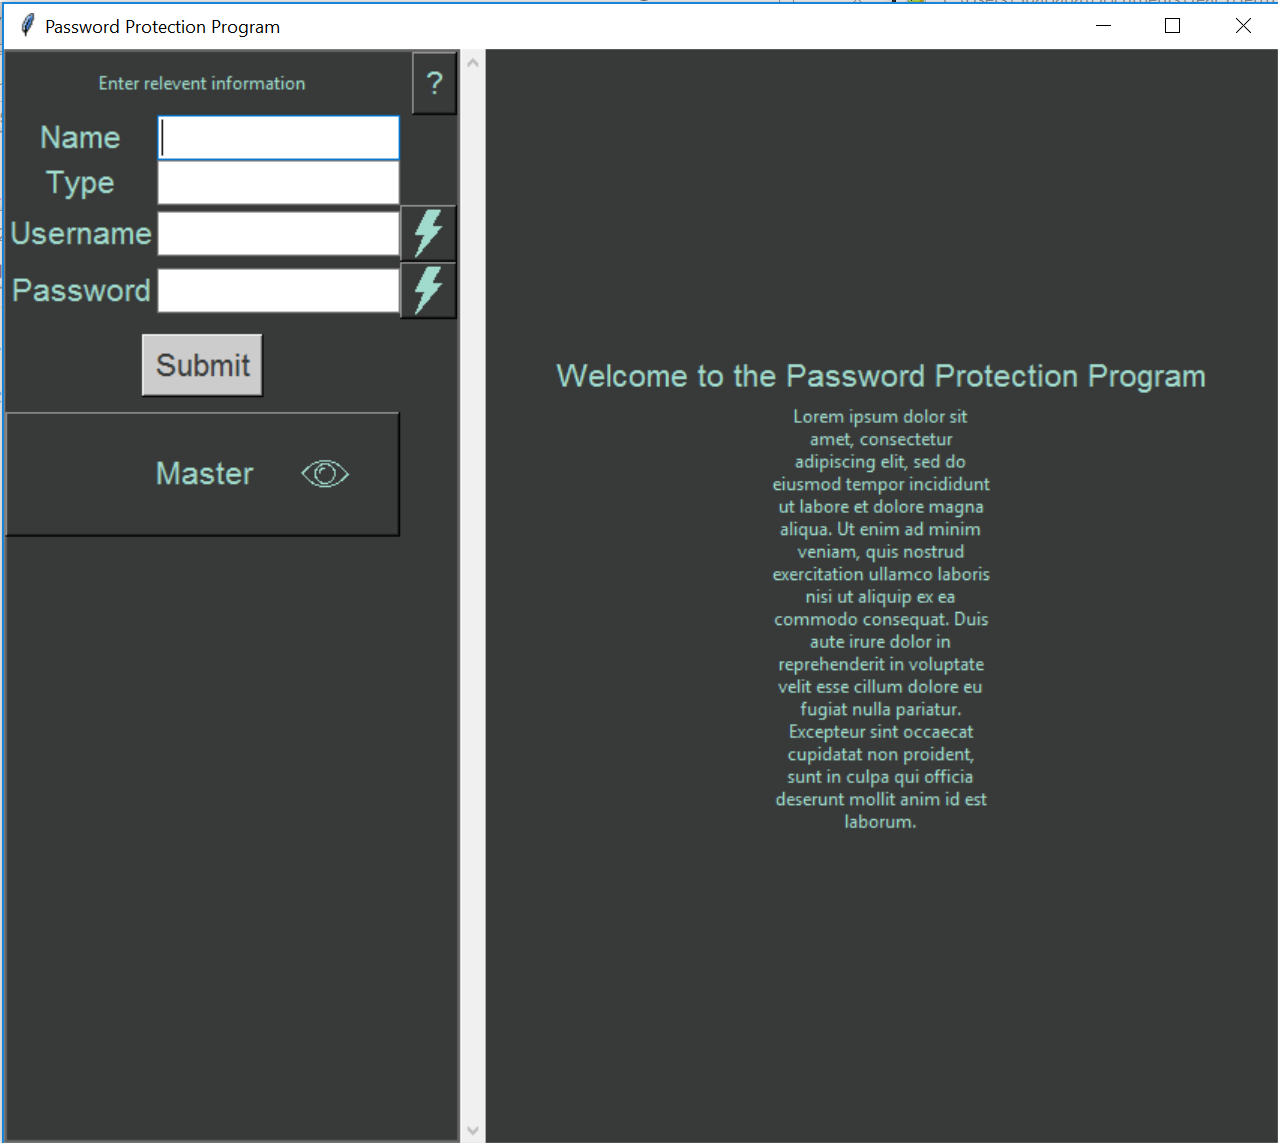
\includegraphics[scale=0.3]{images/InAppScreen.png}
	\caption{In Application Screen}
	\label{fig:InApp}
\end{figure}


\subsection{Changing Master Password} \label{ChangeMasPass}

If the master password that was initially set for the software needs to be changed, this can be done so by choosing the master password box on the left side of the in-application screen.

\begin{figure}[h]
	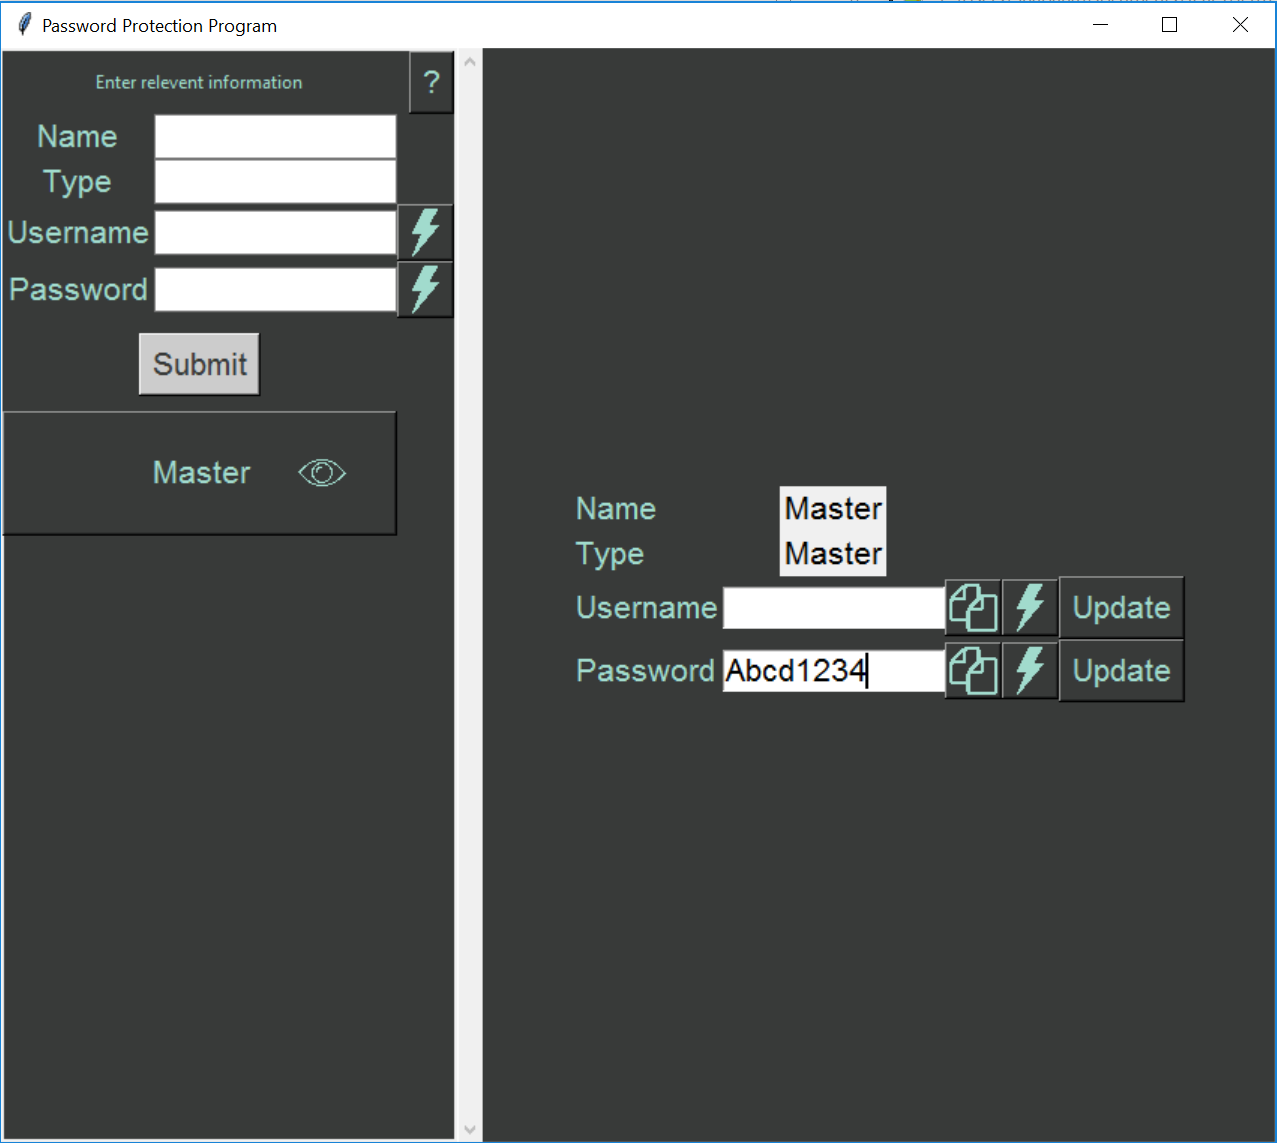
\includegraphics[scale=0.3]{images/ChangeMasPass.png}
	\caption{Changing Master Password}
	\label{fig:chMasPass}
\end{figure}


\subsection{Exit System} \label{SysExit}

The system can be exited by simply closing the application window as this automatically logs the user out as well. The application will also close after TIME AMOUNT of inactivity in order to preserve the security of the data.


\section{Using the System} \label{SysUse}


\subsection{System Functions} \label{SysFunc}

\subsubsection{Add Entry} \label{AddEnt}

\subsubsection{View Entry} \label{ViewEnt}

\subsubsection{Delete Entry} \label{DelEnt}

\subsubsection{Update Entry} \label{UpdateEnt}

\subsubsection{Copy Field} \label{CopyField}

\subsubsection{Generate Field} \label{GenField}

\subsubsection{User Manual} \label{UseMan}


\subsection{Special Instructions for Error Correction} \label{ErrCorr}

TENTATIVE: In the case that the master password is forgotten, the system has a "forgot master password" button that when pressed will reset the application to the state it was when first downloaded. Thus, all saved data will be lost and a new master password will have to be created.


\section{Use Hierarchy Between Modules} \label{SecUse}

In this section, the uses hierarchy between modules is
provided. \citet{Parnas1978} 


%\section*{References}

\bibliographystyle {plainnat}
\bibliography {MG}

\end{document}